\documentclass[tikz,border=0pt,11pt]{standalone}
\usepackage[T1]{fontenc}
\usepackage[utf8]{inputenc}
\usepackage{lmodern,amsmath,amssymb}
\usepackage[swedish]{babel}
\usetikzlibrary{arrows.meta,calc,positioning,decorations.pathmorphing,decorations.pathreplacing,patterns,shadings}
\definecolor{navy}{HTML}{102F40}
\definecolor{teal}{HTML}{147D78}
\definecolor{lightteal}{HTML}{E6F1ED}
\definecolor{gold}{HTML}{B88B3B}
\definecolor{palegold}{HTML}{F7EEDB}
\definecolor{rust}{HTML}{B6533B}
\definecolor{palerust}{HTML}{FAEAE4}
\definecolor{paper}{HTML}{F7F5EE}
\definecolor{muted}{HTML}{5B6D72}
\definecolor{line}{HTML}{D6DED8}
\renewcommand{\familydefault}{\sfdefault}
\newcommand{\atom}[5]{\shade[ball color=#3!70] (#1,#2) circle (#5);\node[text=white,font=\bfseries\small] at (#1,#2){#4};}
\newcommand{\water}[3]{\begin{scope}[shift={(#1,#2)},scale=#3]\draw[navy!45,line width=2pt] (-.3,.22)--(0,0)--(.3,.22);\atom{0}{0}{rust}{O}{.22}\atom{-.3}{.22}{teal}{H}{.15}\atom{.3}{.22}{teal}{H}{.15}\end{scope}}
\newcommand{\panel}[4]{\filldraw[fill=white,draw=line,rounded corners=5pt] (#1,#2) rectangle ++(#3,#4);}
\newcommand{\note}[4]{\node[txt,text width=#3cm] at (#1,#2){#4};}
\tikzset{txt/.style={anchor=north west,align=left,text=navy,font=\small},
 head/.style={anchor=west,text=navy,font=\bfseries\large},
 label/.style={align=center,text=navy,font=\small},
 smalllabel/.style={align=center,text=muted,font=\footnotesize},
 arrow/.style={-{Latex[length=2.5mm,width=1.8mm]},line width=1.2pt,draw=teal},
 goldarrow/.style={-{Latex[length=2.5mm]},line width=1.2pt,draw=gold},
 rustarrow/.style={-{Latex[length=2.5mm]},line width=1.2pt,draw=rust},
 dashedarrow/.style={arrow,dashed},
 badge/.style={fill=lightteal,rounded corners=3pt,text=teal,font=\bfseries\small,inner sep=5pt}}
\begin{document}
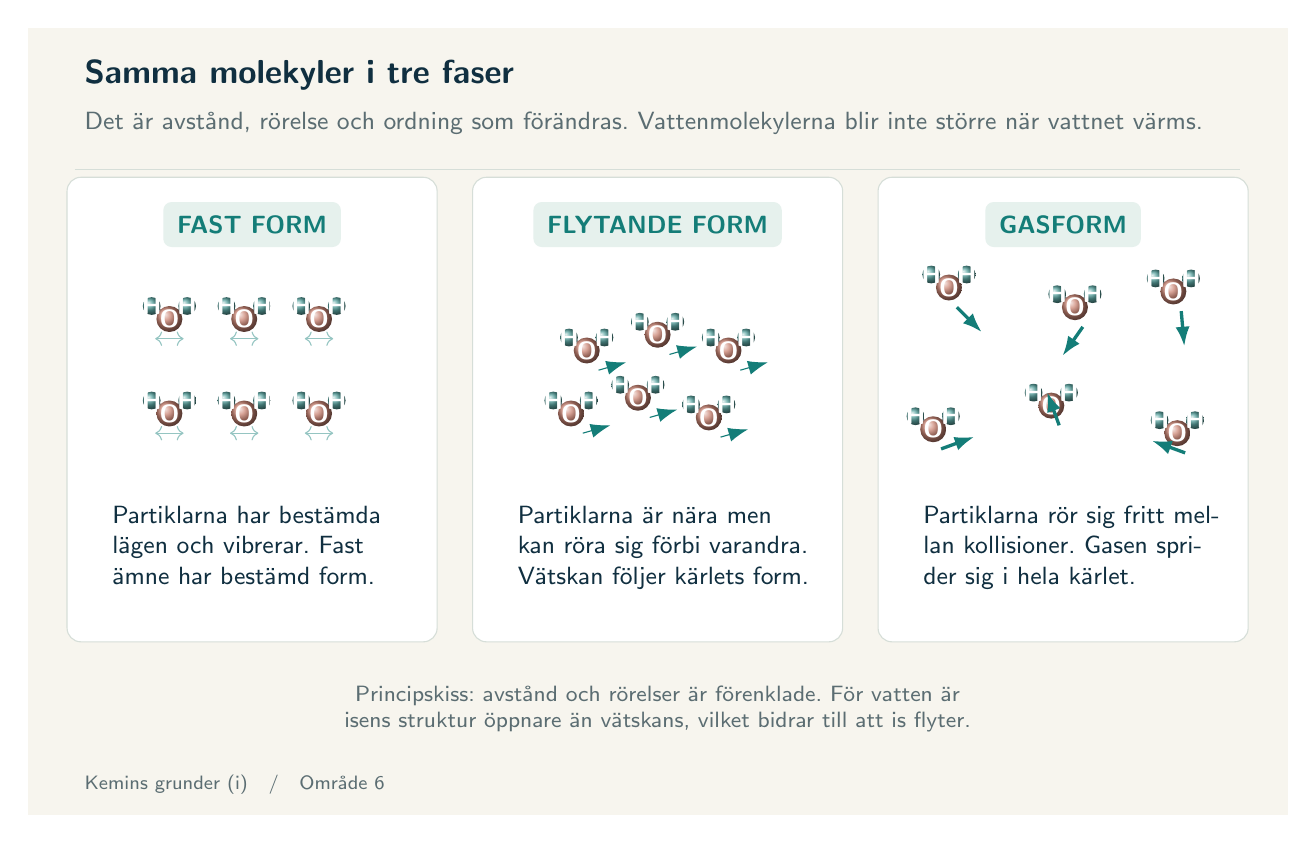
\begin{tikzpicture}[x=1cm,y=1cm]
\path[use as bounding box] (0,0) rectangle (16,10);
\fill[paper] (0,0) rectangle (16,10);
\node[head] at (.6,9.4){Samma molekyler i tre faser};
\note{.6}{9.05}{14.8}{\textcolor{muted}{Det är avstånd, rörelse och ordning som förändras. Vattenmolekylerna blir inte större när vattnet värms.}}
\draw[line] (.6,8.2)--(15.4,8.2);

\foreach \x in {.5,5.65,10.8}{\panel{\x}{2.2}{4.7}{5.9}}
\node[badge] at (2.85,7.5){FAST FORM};\node[badge] at (8,7.5){FLYTANDE FORM};\node[badge] at (13.15,7.5){GASFORM};
\foreach \x in {1.8,2.75,3.7}{\foreach \y in {5.1,6.3}{\water{\x}{\y}{.75}\draw[teal!45,<->] (\x-.18,\y-.25)--(\x+.18,\y-.25);}}
\foreach \x/\y in {6.9/5.1,7.75/5.3,8.65/5.05,7.1/5.9,8/6.1,8.9/5.9}{\water{\x}{\y}{.75}\draw[arrow,thin] (\x+.15,\y-.25)--++(.35,.1);}
\foreach \x/\y/\a in {11.5/4.9/20,13/5.2/110,14.6/4.85/160,11.7/6.7/315,13.3/6.45/235,14.55/6.65/275}{\water{\x}{\y}{.75}\draw[arrow] (\x+.1,\y-.25)--++(\a:.45);}
\note{.95}{4.05}{3.8}{Partiklarna har bestämda lägen och vibrerar. Fast ämne har bestämd form.}
\note{6.1}{4.05}{3.8}{Partiklarna är nära men kan röra sig förbi varandra. Vätskan följer kärlets form.}
\note{11.25}{4.05}{3.8}{Partiklarna rör sig fritt mellan kollisioner. Gasen sprider sig i hela kärlet.}
\node[smalllabel,text width=14cm] at (8,1.35){Principskiss: avstånd och rörelser är förenklade. För vatten är isens struktur öppnare än vätskans, vilket bidrar till att is flyter.};\node[anchor=west,text=muted,font=\scriptsize] at (.6,.38){Kemins grunder (i)\quad /\quad Område 6};

\end{tikzpicture}\end{document}
